\chapter{RISC-V Instruction Formats}

\section{Stored-Program Computer}
\begin{enumerate}
    \item Everything has a memory address: All instructions and data are stored in memory.
    \item Binary compatibility: Programs are distributed in binary form $\implies$ backward-compatible instruction set evolving over time.
\end{enumerate}

\subsection{Instructions as Numbers}
Instructions are 32 bits wide and broken down into different fields.
\begin{itemize}
    \item R-format: register-register arithmetic operations
    \item I-format: register-immediate arithmetic operations and loads
    \item S-format: stores
    \item B-format: branches
    \item J-format: jumps
    \item U-format: 20-bit upper immediate instructions
\end{itemize}

\section{R-Format}
Purpose: register-register arithmetic operations.

\medskip
\begin{tabular}{|c|c|c|c|c|c|}
    \hline
    \texttt{funct7} (7) &
    \texttt{rs2} (5) &
    \texttt{rs1} (5) &
    \texttt{funct3} (3) &
    \texttt{rd} (5) &
    \texttt{opcode} (7) \\
    \hline
\end{tabular}
\begin{itemize}
    \item \texttt{opcode} = 0110011
    \item \texttt{funct7 + funct3}: specifies operation when combined with \texttt{opcode}
    \item Each register holds a 5-bit unsigned integer corresponding to register number (\texttt{x0-31}).
\end{itemize}

\section{I-Format}
Purpose: register-immediate arithmetic operations and loads. Mostly consistent with R-format with \texttt{rs2} and \texttt{funct7} replaced to hold immediates larger than 5 bits.

\medskip
\begin{tabular}{|c|c|c|c|c|}
    \hline
    \texttt{imm[11:0]} (12) &
    \texttt{rs1} (5) &
    \texttt{funct3} (3) &
    \texttt{rd} (5) &
    \texttt{opcode} (7) \\
    \hline
\end{tabular}
\begin{itemize}
    \item \texttt{opcode} = 0010011
    \item \texttt{imm[11:0]}: hold values in range [-2048, 2047]
    \item Immediate is sign-extended to 32-bits before use.
\end{itemize}

\subsection{Loads}
Load instructions are also I-type with the \texttt{imm} field encoding the offset in bytes.

\medskip
\begin{tabular}{|c|c|c|c|c|}
    \hline
    \texttt{offset[11:0]} (12) &
    \texttt{base} (5) &
    \texttt{width} (3) &
    \texttt{dest} (5) &
    \texttt{LOAD} (7) \\
    \hline
\end{tabular}
\begin{itemize}
    \item \texttt{opcode} = 0000011
    \item \texttt{width}: refers to the size and sign of load data
    \begin{itemize}
        \item bit 1: 0 = signed; 1 = unsigned
        \item bits 2-3: 00 = 1 byte; 01 = 2 bytes; 10 = 4 bytes
    \end{itemize}
\end{itemize}

\section{S-Format}
Purpose: stores. Need to read two source registers but no destination. We want to prioritize keeping registers in the same place so \texttt{imm} field is split (8 + 4).

\medskip
\begin{tabular}{|c|c|c|c|c|c|}
    \hline
    \texttt{imm[11:5]} (7) &
    \texttt{rs2} (5) &
    \texttt{rs1} (5) &
    \texttt{funct3} (3) &
    \texttt{imm[4:0]} (5) &
    \texttt{opcode} (7) \\
    \hline
\end{tabular}
\begin{itemize}
    \item \texttt{opcode} = 0100011
    \item \texttt{rs1}: base memory 
    \item \texttt{rs2}: data to be stored
\end{itemize}

\section{B-Format}
Purpose: branches. Need to read two registers but no destination (similar to stores).

Instructions are stored in localized code memory. The address of current instruction is stored in the PC $\implies$ use \emph{PC-relative addressing} by storing offset in \texttt{imm}:
\begin{itemize}
    \item If we don't branch: PC += 4
    \item If we branch: PC += 2 \(\times\) immediate
    \item With 12 bits, we can specify $\pm 2^{11}$ bytes away from the PC.
    \item Instructions are 4 bytes $\implies$ we can jump $\pm 2^9$ instructions away from current instruction.
\end{itemize}

\subsection{RISC-V Feature: nx16-bit Instructions}
RISC-V supports 16-bit compressed instructions by scaling the branch offset by 2 bytes when there are no 16-bit instructions.
\begin{itemize}
    \item Range of bytes we can jump to: \(\pm 2^{12}\)
    \item Range of 32-bit instructions we can jump to: \(\pm 2^{10}\)
\end{itemize}

\medskip
\begin{tabular}{|c|c|c|c|c|c|}
    \hline
    \texttt{imm[12|10:5]} (1|6) &
    \texttt{rs2} (5) &
    \texttt{rs1} (5) &
    \texttt{funct3} (3) &
    \texttt{imm[4:1|11]} (4|1) &
    \texttt{opcode} (7) \\
    \hline
\end{tabular}
\begin{itemize}
    \item \texttt{opcode} = 1100011
    \item \texttt{imm[12:1]}: represents values \([-4096, 4096]\) in 2-byte increments
    \item Lowest bit of offset is always 0 (since address is always even) so we do not store it.
    \item Example (branch offset): In this loop, the branch offset to \texttt{End} is 4 instruction \(\implies\) (4 instructions \(\times\) 4 bytes) = 16 bytes.
        \begin{minted}{asm}
        Loop:  beq x19, x10, End
               add x18, x18, x10
               addi x19, x19, -1
               j Loop
        End:   # target
    \end{minted}
\end{itemize}

\section{J-Format}
Purpose: jumps.

\medskip
\begin{tabular}{|c|c|c|}
    \hline
    \texttt{imm[20|10:1|11|19:12]} (1|10|1|8) &
    \texttt{rd} (5) &
    \texttt{opcode} (7) \\
    \hline
\end{tabular}
\begin{itemize}
    \item \texttt{opcode} = 1101111
    \item \texttt{imm[20:1]}: can jump by \(\pm 2^{20}\) bytes or \(\pm 2^{18}\) 32-bit instructions
    \item Lowest bit of offset is always 0.
    \item JAL saves PC + 4 in register \texttt{rd}.
\end{itemize}

\subsection{JALR}
JALR is \underline{I-type}.

\medskip
\begin{tabular}{|c|c|c|c|c|}
    \hline
    \texttt{imm[11:0]} (12) &
    \texttt{rs1} (5) &
    \texttt{funct3} (3) &
    \texttt{rd} (5) &
    \texttt{opcode} (7) \\
    \hline
\end{tabular}
\begin{itemize}
    \item \texttt{opcode} = 1100111
    \item Sets PC = \texttt{rs} + \texttt{immediate}
    \item Uses same immediates as arithmetic and loads: NO multiplication by 2 bytes.
    \item Unlike JAL, we include the last 0th bit because JALR is I-type.
\end{itemize}

\section{U-Format}
Purpose: upper immediates.

\medskip
\begin{tabular}{|c|c|c|}
    \hline
    \texttt{imm[31:12]} (20) &
    \texttt{rd} (5) &
    \texttt{opcode} (7) \\
    \hline
\end{tabular}
\begin{itemize}
    \item To create any 32-bit value, \texttt{lui} loads the upper 20 bits of the destination then \texttt{addi} sets the lower 12 bits.
    \item \texttt{auipc} adds a 20-bit int to PC.
\end{itemize}

\medskip
\begin{figure}[H]
  \centering
  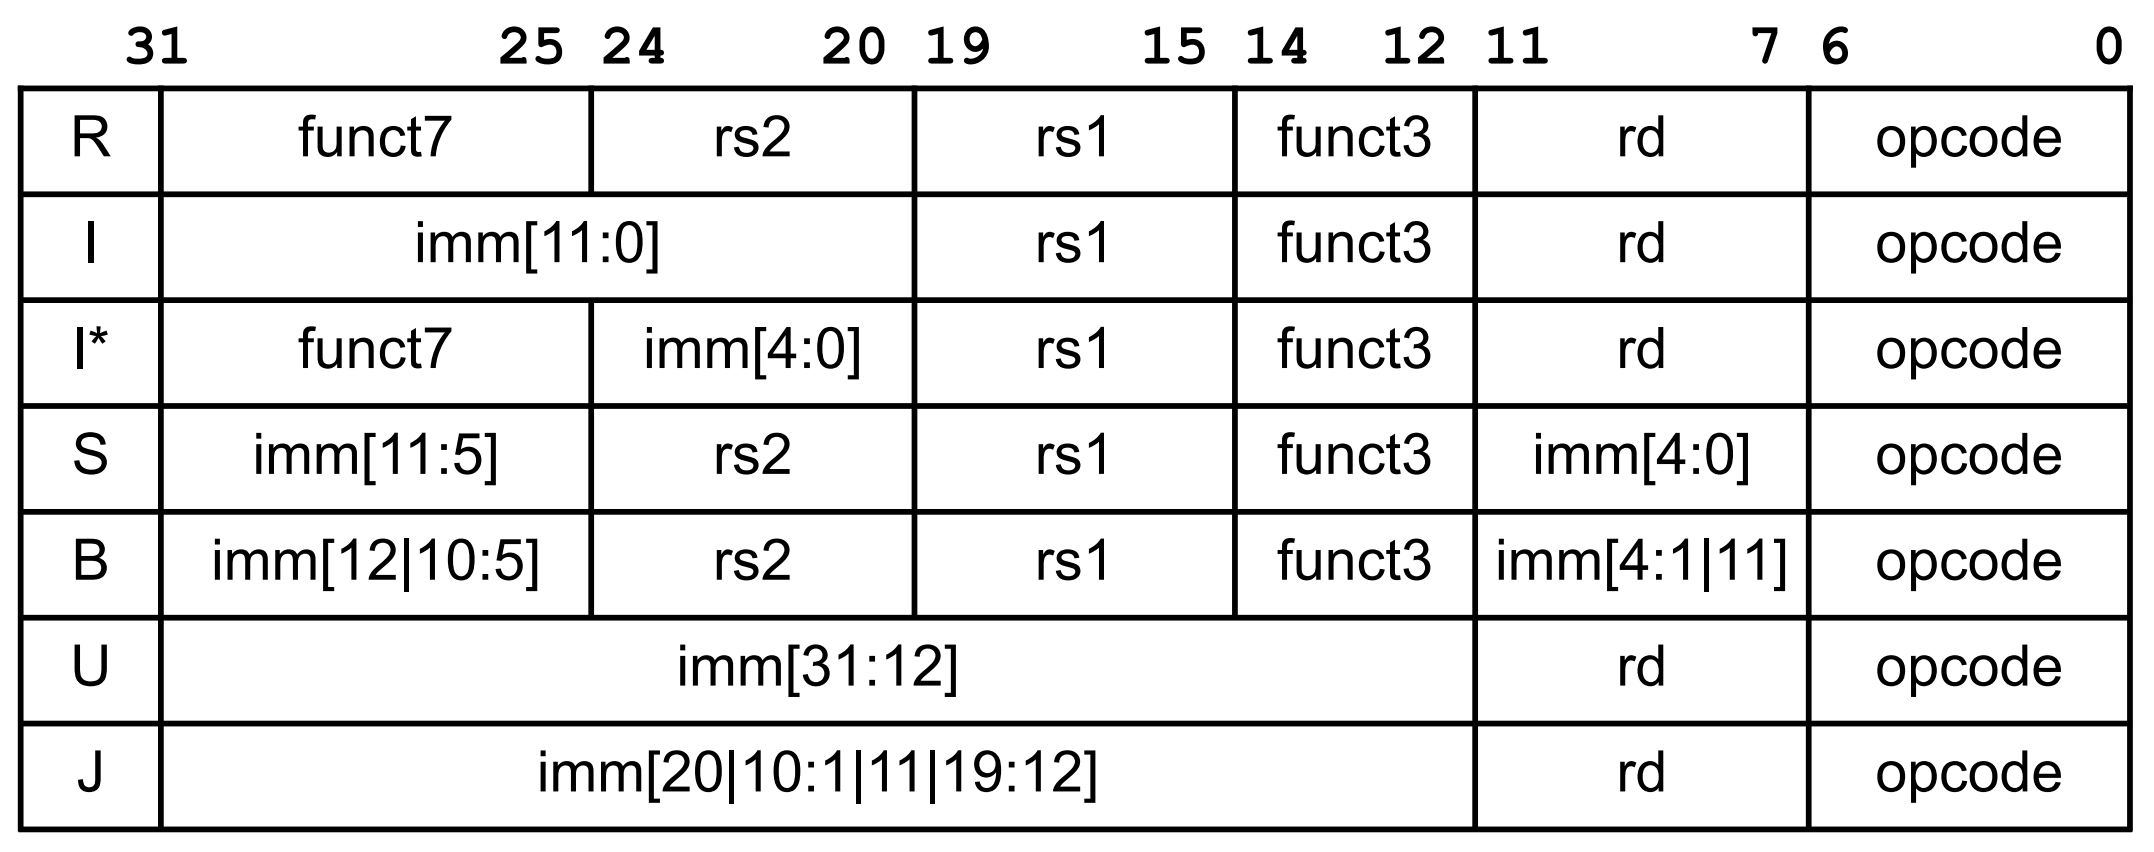
\includegraphics[width=1\linewidth]{figures/riscv-instructs}
  \caption{RISC-V instruction formats.}
\end{figure}